% Created 2023-08-10 Thu 11:44
% Intended LaTeX compiler: pdflatex
\documentclass[11pt]{article}
\usepackage[utf8]{inputenc}
\usepackage[T1]{fontenc}
\usepackage[a4paper, margin=3cm]{geometry}
\usepackage{graphicx}
\usepackage{longtable}
\usepackage{wrapfig}
\usepackage{rotating}
\usepackage[normalem]{ulem}
\usepackage{amsmath, amssymb, amsthm}
\usepackage{capt-of}
\usepackage{hyperref}
\author{Lokesh Mohanty}
\date{\today}
\title{Advanced Deep Representation Learning}
\hypersetup{
  pdfauthor={Lokesh Mohanty},
  pdftitle={Advanced Deep Representation Learning},
  pdfkeywords={},
  pdfsubject={},
  pdfcreator={Emacs 29.0.60 (Org mode 9.7-pre)}, 
  pdflang={English}}

\setlength\parindent{0pt}
\usepackage{enumerate}
\usepackage{framed}
\usepackage{import}
\usepackage{xcolor}
\usepackage{transparent}
\DeclareMathOperator*{\E}{\mathbb{E}}

\usepackage[onehalfspacing]{setspace}
\newtheorem{theorem}{Theorem}[section]
\newtheorem{corollary}{Corollary}[theorem]
\newtheorem{lemma}[theorem]{Lemma}

\usepackage{tikzit}
\input{sample.tikzstyles}
\usepackage{caption}

\begin{document}

\maketitle
\tableofcontents

\clearpage
\section{Latent Variable Models \\and Variational Inference}
\label{sec:org1db23b0}

\paragraph{Generative Modelling:}
Given $\mathcal{D} = \left( \left\{ x_1, x_2, ..., x_n \right\} \right) \sim i.i.d. \mathcal{P}_x$
$\left( \Omega, \mathcal{F}, \mathcal{P} \right) \rightarrow \left( \mathcal{R}, B, \mathcal{P}_x \right)$,
estimate $P_x$ and sample from it.

\subsection{Density Estimation (Estimate $P_x$)} 
\label{sec:density-estimation}

Suppose $\mathcal{P}_x$ is the unknown density function.
\vspace{1em}

Let $P_{\theta}$ be an estimate of $P_x$
\textit{(Any function on data can be considered as an estimate)}
\vspace{1em}

\textbf{Objective}: Get $P_{\theta}$ \underline{close} to $P_x$.

Define closeness between densities: KL divergence ($\mathcal{D}_{KL}$) (one possibility)

Given two density functions $P_{\theta}, P_x$, correspondint to a continuous random variable (CRV) $X$, then
\begin{align*}
  \mathcal{D}_{KL}\left( P_x || P_{\theta} \right) \triangleq \int_X P_x(x) log \frac{P_x(x)}{P_{\theta}(x)} dx
\end{align*}

$P_{\theta}$ is a parametric function of $\mathcal{D}$, parameterized by $\theta$.

$\therefore$ Estimating $P_{\theta}$ is equivalent to estimating $\theta$.
\vspace{1em}

One estimate for $\theta$:
\begin{align*}
  \theta^{*} = \arg\min_{\theta} \left\{ \mathcal{D}_{KL} \left[ P_x || P_{\theta} \right] \right\} \quad\text{(Maximum likelihood estimate)}
\end{align*}
\vspace{1em}

The reason we consider $\mathcal{D}_{KL}(P_x || P_{\theta})$ instead of $\mathcal{D}_{KL}(P_{\theta} || P_x)$ is
\begin{align*}
  \mathcal{D}_{KL} \left( P_x || P_{\theta} \right) &= \int P_x log \frac{P_x}{p_{\theta}} dx \\
                                                    &= \int P_x log P_x dx - \int P_x log P_{\theta} dx \\
  \min_{\theta} \mathcal{D}_{KL}(P_x || P_{\theta}) &\cong \min_{\theta} \left( - \int P_x log P_{\theta} dx \right) \\
\end{align*}

Suppose $x$ is a CRV and $f(x)$ is any function on $x$, $f(x) : x \rightarrow \mathbb{R}$

if $P_x$ is the density of $x$,
\begin{align*}
  \mathop{\mathbb{E}}_x &= \int_x x P_x(x) dx, \\
  \mathop{\mathbb{E}}_{f(x)} &= \int_{f(x)} f(x) P_{f(x)}\left( f(x) \right) df(x), \\
                        &= \int_x f(x) P_x dx \quad\text{(LOTUS)}
\end{align*}

From this,
\begin{align*}
  -\int P_x log P_{\theta} (x) dx &\rightarrow -\int P_x (f(x)) dx
                                    = \mathop{\mathbb{E}}_x \left( -log P_{\theta}(x) \right) \\
                                  &\sim - \frac{1}{n} \sum_{i=1}^n log P_{\theta}\left( x_i \right) \quad\text{(From Weak law of large numbers (W.L.L.N))}
\end{align*}
\vspace{1em}

$P_{\theta}(x_i)$ is the likelihood of $x_i$ under $P_{\theta}$ (it is not a probability)
\vspace{1em}

Let \(P_{\hat{\theta}}\) be an estimate of
\begin{align*}
  P_{x_1, x_2, ..., x_n}(x_1, x_2, ..., x_n) &= \mathop{\Pi}_{i=1}^n P_{x_i}(x_i) \\
  P_{\hat{\theta}} (\mathcal{D}) &= \mathop{\Pi}_{i=1}^n P_{\theta}(x_i) \\
  \theta^{*} &= \arg\max_{\theta} \mathop{\Pi}_{i=1}^n P_{\theta}(x_i)
\end{align*}
\vspace{1em}

\subsubsection{ML estimation for Mixture Densities}
\label{sec:ml-estim-mixt}

Choosing $P_{\theta}$ is a design choice. Choosing ``wrong'' $P_{\theta}$ leads to large $\mathcal{D}_{KL}$
\begin{itemize}
\item Make $P_{\theta}$ expressive enough: choose $P_{\theta}$ from universal approximators. \\
  \textbf{Eg}: Mixture Density $P_{\theta}(x_i) = \sum_{j=1}^M \alpha_j P_{\alpha_j} (x_i)$, $\sum_{j=1}^M \alpha_j = 1$
\end{itemize}

For an M-component GMM,
\[ \theta = \left\{ \alpha^M, \mu|_{d \times 1}^M, \sum|_{d \times d}^M \right\} \]

\begin{align*}
  \theta^{*}_{ML} &= \arg\max_{\theta} \sum_{i=1}^Mlog P_{\theta}(x_i) \\
                  &= \arg\max_{\alpha, \mu, \Sigma} \sum_{i=1}^M \alpha_j \text{exp}((x_i - \mu_j)^T\Sigma_j^{-1}(x_i - \mu_j)) \\
                  & \text{(Intractable)}
\end{align*}



There exists a latent/hidden variable in data that is unobserved. In latent variable modelling, we try to model this hidden variable. To do this, we introduce another random variable $z \in Z$ such that

\begin{align*}
  D_c &= \left\{ (x_1, z_1), (x_2, z_2), \dots, (x_n, z_n) \right\} \sim \text{i.i.d } \mathbb{P}_{xz} \\
  D &= \left\{ x_i \right\}^n_{i=1} \sim \text{i.i.d } \sum_z P_{xz}
\end{align*}

Suppose $D$ was sampled as follows:
There are M Gaussian distributions
\begin{enumerate}[(i)]
\item Throw a die, $z \sim $ discrete M-faced die ($\Pi_z(\alpha_1, ..., \alpha_n)$)
\item Pick a Gaussian depending upon the outcome of (i)
\item Sample a datapoint from that Gaussian
\end{enumerate}

Outcome: $\left\{ x_1, x_2, ..., x_n \right\}$ \\

When we do sampling from a mixture density, we sample from the conditional(design choice) while for estimating, we consider the marginal density. \\

\begin{minipage}{0.45\textwidth}
  \begin{framed}
    \centering
    Sample $z_i \sim \Pi_z$ \\
    Sample from $P_{x|z = z_i}$ \\
  \end{framed}
\end{minipage}

\clearpage
\paragraph{Maximum Likelihood estimation  for LVM:}

\begin{align*}
  P_{\theta}(x) &= \int_z P_{\theta}(x, z) dz \\
                &= \int_z \frac{P_{\theta}(x, z)}{q(z)}q(z) dz\,, \quad\text{where $q(z)$ is any arbitrary density on $z$} \\
  \implies \log P_{\theta}(x) &= \log \int_z P_{\theta}(x, z) dz \\
                &= \log\int_z \frac{P_{\theta}(x, z)}{q(z)}q(z) dz \\
                &= \log \E_{q(z)} \frac{P_{\theta}(x,z)}{q(z)}
                  \geq \E_{q(z)} \log \frac{P_{\theta}(x, z)}{q(z)} \\
                &= \int q(z) \log \frac{P_{\theta}(x, z)}{q(z)} dz \\
                &= \E_{q(z)}\log P_{\theta}(x, z) + \left( -\int q(z) \log q(z)dz \right) \\
  \implies \log P_{\theta}(x) &\geq \E_{q(z)}\log P_{\theta}(x, z) + H(q) \\
  \implies \log P_{\theta}(x) &\geq F_{\theta}(q) \rightarrow \text{Evidence lower bound (ELBO)} \\
  \text{likelihood } P_{\theta}(x) &: \text{Evidence}
\end{align*}

Here $q(z)$ is called the variational density. \\
\textbf{Question}: What $q(z)$ tightens the ELBO? \\
When it is an estimate for $P(z|x=x_i)$.

\begin{align*}
  F_{\theta}(q) &= \E_{q(z)} \log \frac{P_{\theta}(x, z)}{q(z)} 
\end{align*}

\textbf{22nd August 2023}
\subsection{Iterative ELBO Optimization (EM algorithm)}
\label{sec:iter-elbo-optim}

\textbf{Question:} Why is optimizing ELBO useful/correct? How to optiimze it?

\vspace{1em}
Mazimize $F_{\theta}(q)$ w.r.t. $q(z)$ for a given $\theta$. (E-step)
\begin{align*}
  Q^{t+1}(z) &= \arg\max_{q(z)} F_{\theta^t}(q(z))
\end{align*}

Mazimize $F_{\theta}(q)$ w.r.t. $\theta$ for a given $q$. (M-step)
\begin{align*}
  \Theta^{t+1} &= \arg\max_{\theta} F_{\theta}(Q^{t+1})
\end{align*}

Stopping criteria:
\begin{align*}
  |l(\theta^{t+1}) - l(\theta^t)| < \epsilon, \quad \text{where $l(\theta)$ is log likelihood of $P_{\theta}(x)$}
\end{align*}

\begin{lemma}
  For EM algorithm, $l(\theta^{t+1}) \geq l(\theta^t)$
\end{lemma}

\begin{proof}
  Consider,
  \begin{align*}
    l(\theta) - F_{\theta}(q) &= \log P_{\theta}(x) - \int_z q(z) \log \frac{P_{\theta}(x, z)}{q(z)}dz \\
                              &= \log P_{\theta}(x) - \int_z q(z) \log \frac{P_{\theta}(z|x)P_{\theta}(x)}{q(z)}dz \\
                              &= \log P_{\theta}(x) - \log P_{\theta}(x) + \int_z q(z) \log \left[ \frac{q(z)}{P_{\theta}(z|x)} \right]dz \\
                              &= D_{KL} \left( q(z) \Vert P_{\theta}(z|x) \right) \\
    \implies l(\theta) &= F_{\theta}(q) \quad\text{if}\quad q(z) = P_{\theta}(z|x) \\
    \implies \arg\max_q F_{\theta}(q) &= P_{\theta}(z|x)
  \end{align*}

  Therefore,
  \begin{align*}
    F_{\theta}(q) &\leq l(\theta), \quad F_{\theta}(q) = l(\theta) \quad\text{for } q(z) = P_{\theta}(z|x)
  \end{align*}

  In E-step, $q^{t+1}(z) = P_{\theta^t}(z|x)$ $\implies l(\theta^t) = F_{\theta^t}(q^{t+1})$,\\
  In M-step, $F_{\theta^{t+1}}(q^{t+1}) \geq F_{\theta^t}(q^{t+1})$

  We have $F_{\theta^{t+1}}(q^{t+1}) \leq l(\theta^{t+1})$ [Jenson's inequality by construction] \\
  $\therefore l(\theta^{t+1}) \geq l(\theta^t)$
\end{proof}

\subsection{EM for Mixture Densities}
\label{sec:em-mixture-densities}

\begin{align*}
  P_{\theta}(x) &= \sum_z P_{\theta}(x, z) = \sum_z P_{\theta}(x|z)P_{\theta}(z)
\end{align*}

For GMM,
\begin{align*}
  P_{\theta}(x | z) &\sim \mathcal{N}\left( x_i, \mu_n, \Sigma_n \right) \\
  P_{\theta}(z) &\sim \text{Disc} \left( 1, ..., M \right) \\
                    &\text{with probability: } \alpha_1, \alpha_2, ..., \alpha_n \\
                    &\text{where, } \alpha_m \geq 0, \sum_{m=1}^M\alpha_m = 1
\end{align*}

E - step: Compute $P_{\theta}(z|x)$,
\begin{align*}
  P_{\theta}(z|x) &= \frac{P_{\theta}(x|z) P_{\theta}(z)}{P_{\theta}(x)} = q^{t+1}
\end{align*}

M - step: Compute $F_{\theta}(q)$,
\begin{align*}
  F_{\theta}(q) &= \E_{q^{t+1}} \log \frac{P_{\theta}(x, z)}{q^{t+1}(z)} \\
                &= \E_{P_{\theta^t}(z|x)} \log \frac{P_{\theta}(x, z)}{P_{\theta^t}(z|x)} \\ 
                &= \E_{P_{\theta^t}(z|x)} \log P_{\theta}(x, z) + \underbrace{H(P_{\theta^t}(z | x))}_{\text{independent of } \theta} \\
  \implies \theta^{t+1} &= \arg\max_{\theta} \E_{P_{\theta^t}(z|x)} \log P_{\theta}(x, z)
\end{align*}


\textbf{24th August 2023}\vspace{1em}

\begin{framed}
  Parts of any Machine Learning model:
  \begin{enumerate}[(i)]
  \item Modelling (Training)
  \item (Posterior) Inference (Testing/Validation) $\rightarrow$ (Evaluate $P(y|X = X_{\text{test}})$) \\
    (In latent variable models $\rightarrow$ evaluate $P(z|x)$)
  \item Sampling (Only for generative models)
  \end{enumerate}
\end{framed}

\vspace{1em}
For GMM:
\begin{itemize}
\item Modelling: Estimate $\alpha$, $\mu$, $\Sigma$ via EM(KL minimization)
\item Inference: Given $X_{\text{test}}$, evaluate $P(z|X_{\text{test}})$
\end{itemize}

\vspace{1em}
Sampling from GMM
\begin{enumerate}
\item\label{item:4} Sample $z_i = m \sim \text{Dis}(1, ..., \mu)$ with probability ($\alpha_1, ..., \alpha_M$)
\item\label{item:5} Sample $x_i$ from $P(x_i | z_i=m) \sim \mathcal{N}(x, \mu_m^{*}, \Sigma_m^{*})$
\end{enumerate}

\section{Auto-Encoding Variational Bayes \\(Variational Auto-Encoders)}
\label{sec:auto-encod-vari}

Given $\mathcal{D} = \left\{ x_1, ..., x_n \right\} \sim \text{ i.i.d } \mathbb{P}_x$ \\
Let $P_{\theta}$ be the model density

\underline{Objectives:}
\begin{enumerate}[(i)]
\item\label{item:1} obtain ML estimate (for $P_x$)
\item\label{item:2} perform posterior inference (evaluate $P(z|x)$)
\item\label{item:3} sample (from $P_x$)
\end{enumerate}

\begin{framed}
  Issues with Mixture Models ($P_{\theta}$) 
  \begin{itemize}
  \item  Need to estimate $P_{\theta}(z | x)$
  \item EM saturates, with high dimensional data
  \end{itemize}
\end{framed}

Requirement: A model for $P_{\theta}$ without the need to compute $P(z|x)$ explicitly
\vspace{1em}

\textbf{29th August 2023}

We have
\[ l(\theta) \geq F_{\theta}(q) = \E_q \log \frac{P_{\theta}(x, z)}{q(z)} \]

Let variational distribution be $q(z|x)$ (posterior)

\begin{align*}
  F_{\theta}(q) &= \E_{q(z|x)} \log \frac{P_{\theta}(x, z)}{q(z|x)} \\
                &= \E_{q(z|x)} \log \frac{P_{\theta}(x|z)P_{\theta}(z)}{q(z|x)} \\
                &= \E_{q(z|x)} \log P_{\theta}(x|z) - \int_z q(z|x) \log \left[ \frac{q(z|x)}{P_{\theta}(z)} \right] dz \\
                &= \E_{q(z|x)} \log P_{\theta}(x|z) - D_{KL}\left[ q(z|x) \Vert P_{\theta}(z)) \right]
\end{align*}

Parameterize $P_{\theta}(x|z)$ and $q(z|x)$ using neural networks with parameters $\theta$ and $\phi$ respectively. In the above equation, we assume $P_{\theta}(z)$ to be $P(z)$ i.e., independant of $\theta$ to make it easy to backpropagate.

\vspace{1em}

for $F_{\theta}(q_{\phi})$, we need $\nabla_{\phi}F_{\theta}(q_{\phi})$ and $\nabla_{\theta}F_{\theta}(q_{\phi})$

\vspace{1em}

Consider the first term (data conditional log likelihood) in ELBO, ($\theta$ has the generative parameters)
\begin{align*}
  \nabla_{\phi, \theta}\E_{q_{\phi}(z|x)} \log P_{\theta} (x | z)
\end{align*}

This looks like ($\psi = \{\phi, \theta\}$)
\[\E_{P_v} f_{\psi}(v), \quad v \sim P_v\]

We need
\begin{align*}
  \nabla_{\psi} \E_{P_v} \left[ f_{\psi}(v) \right] &= \nabla_{\psi} \int_v P_v(v)f_{\psi}(v)dv \\
                                                    &= \int_v\nabla_{\psi} P_v(v)f_{\psi}(v) dv \\
                                                    &= \int_v P_v(v) \nabla_{\psi} f_{\psi}(v) dv \\
                                                    &= \E_{P_v} \nabla_{\psi}f_{\psi}(v)
\end{align*}

By \textbf{Monte-Carlo gradient estimates} (W. L. L. N.),
\begin{align*}
  \nabla_{\psi}\E_{P_v} f_{\psi}(v) &\approx
                                      \frac{1}{N} \sum_{i=1}^N \nabla_{\psi}f_{\psi}(v_i), \quad \left\{ v_i \right\}^k_{i=1} \sim i.i.d. P_v
\end{align*}

In our case though, we have
\begin{align*}
  \nabla_{\psi} \E_{P_{\psi}(v)} \left[ f_{\psi}(v) \right] &= \int_v \nabla_{\psi}\left\{ P_{\psi}(v).f_{\psi}(v) \right\}dv \\
                                                            &= \underbrace{\int_v f_{\psi}(v) . \nabla_{\psi} P_{\psi}(v) dv}_{\substack{\text{not an expectation} \\ \text{and thus can't get} \\ \text{MC estimates}}}
  + \underbrace{\int_v P_{\psi}(v). \nabla_{\psi} f_{\psi}(v)dv}_{\substack{\E_{P_{\psi}(v)}\nabla_{\psi}f_{\psi}(v) \\ \text{can be evaluated using} \\ \text{MC estimates}}}
\end{align*}

The \textbf{Reparameterization} Trick: \\
We need $\nabla_{\psi}\E_{P_{\psi}(v)}f_{\psi}(v)$ \\
Suppose $\exists$ a deterministic function $g: \epsilon \rightarrow v$, where $\epsilon$ is any arbitrary random variable with a density $P_{\epsilon}$, i.e., $v = g_{\psi}(\epsilon)$

\begin{align*}
  \E_{P_{\psi}(v)} f_{\psi}(v)
  &= \E_{P_{\epsilon}}\left[ f_{\psi}\left( g_{\psi}(\epsilon) \right) \right] \\
  \implies \nabla_{\psi}\E_{P_{\psi}(v)}f_{\psi}(v)
  &= \nabla_{\psi} \E_{P_{\epsilon}} \left[ f_{\psi}\left( g_{\psi}(\epsilon) \right) \right] \\
  &= \E_{P_{\epsilon}} \nabla_{\psi} \left[ f_{\psi}\left( g_{\psi}(\epsilon) \right) \right] \\
  &\approx \frac{1}{L} \sum_{i=1}^L \nabla_{\psi} \left[ f_{\psi}\left( g_{\psi}(\epsilon_i) \right) \right],
    \quad \epsilon_i \sim \text{ i.i.d } P_{\epsilon}
\end{align*}

\begin{framed}
  \textbf{Example for Reparameterization:} \\
  Suppose $v \sim \mathcal{N}(v, \mu, \sigma^2)$
  \begin{align*}
    v &= \mu + \sigma\epsilon, \quad \epsilon \sim \mathcal{N}(0, I) \\
    g(\epsilon) &= \mu + \sigma\epsilon
  \end{align*}
\end{framed}

\textbf{31st August 2023}

Encoder Network ($\phi$) for $Q(z|x)$ $\rightarrow$ probabilistic \\
Decoder Network ($\theta$) for $P(z|x)$ $\rightarrow$ deterministic \\


Assumption: \\
$Q(z|x) \sim \mathcal{N}(z, \mu_x, \Sigma_x)$ \\
$D = \left\{ x_1, ..., x_n \right\}^n_{i=1} \sim \mathbb{P}_x$,
$x_i \in \mathbb{R}^d$, $Z \in \mathbb{R}^k$, $k \ll d$


\begin{figure}[h]
  \begin{minipage}{0.45\textwidth}
    \centering
    \def\svgwidth{\columnwidth}
    \subimport{figures}{vae_encoder.pdf_tex}
    \caption{Encoder}
    \label{fig:vae-encoder}
  \end{minipage}%
  \begin{minipage}{0.45\textwidth}
    \centering
    \def\svgwidth{\columnwidth}
    \subimport{figures}{vae_decoder.pdf_tex}
    \caption{Decoder}
    \label{fig:vae-decoder}
  \end{minipage}%
\end{figure}

\clearpage
\vspace{1em}
For training the decoder:

Train $\phi$ and $\theta$ via minimizing the negative ELBO
\begin{align*}
  \phi^{t+1}, \theta^{t+1} &= \phi^t, \theta^t - \alpha \nabla_{\phi, \theta}\left( -F_{\theta}(q_{\phi}) \right)
\end{align*}

Consider
\begin{align*}
  \E_{q(z|x)} \log P_{\theta}(x | z) &\cong \frac{1}{L} \sum_{l=1}^L \log P_{\theta}(x | g(\epsilon_l)), \quad \epsilon_l \sim P_{\epsilon} \\
  g(t) &= M + t \cdot \Sigma, \quad z = g(\epsilon_l) \\
  z_i^l &= M_{x_i} + \epsilon_l \cdot \Sigma_{x_i}
\end{align*}

One way of computing $\log P_{\theta}(x | z)$. Assume
\begin{align*}
  P_{\theta}(x | z) &\sim \mathcal{N}(x; \hat{x}, I) \\
  \implies \log P_{\theta}(x | z) &\propto \Vert x - \hat{x} \Vert_2^2 \\
  \implies \E_{q_{\phi}(z | x)} \log P_{\theta}(x | z) &\approx
                                                         - \sum_{l = 1}^L \Vert X - \hat{X}_{\phi, \theta}^l \Vert^2_2
\end{align*}

For training the encoder:
\begin{align*}
  D_{KL} \left[ q_{\phi}(z|x) \Vert P(z) \right] &\approx \frac{1}{2} \left[ tr(\Sigma^{\phi}) + \mu_x^{\phi T}\mu_x^{\phi} - K - \log |\Sigma^{\phi}| \right]
\end{align*}

Therefore,
\begin{align*}
  F_{\theta}(q_{\phi}) &= \E_{q(z|x)} \log P_{\theta}(x | z) - D_{KL} \left[ q_{\phi}(z|x) \Vert P(z) \right] \\
                       &\approx \Vert x - \hat{x} \Vert_2^2 + \frac{1}{2} \left[ tr(\Sigma^{\phi}) + \mu_x^{\phi T}\mu_x^{\phi} - K - \log |\Sigma^{\phi}| \right]
\end{align*}

\vspace{1em}
Steps: Training VAE, Sampling/Generation with VAE, Remove the encoder \\

Sample $z \sim P(z)$. Decoder is expected to output $\tilde{x} \sim P_{\theta}(x | z)$.
\begin{align*}
  \therefore D_{KL} \left[ q_{\phi}(z | x) \Vert P_{\theta}(z) \right] \quad\text{is minimized}
\end{align*}

\subsection{VAE as a regularized auto encoder}
\label{sec:vae-as-regularized}

Learn to sample from $z \sim q(z)$

\begin{align*}
  L_{AE} &= \Vert x - \hat{x}\Vert_2^2 + \underbrace{D_{KL}(q_2() \Vert P_z)}_{\text{regularizer on $z/q_z$}}
\end{align*}

\textbf{Posterior Inference:}

Consider the encoder:

% \begin{figure}
%   \centering
%   \def\svgwidth{\columnwidth}
%   \subimport{figures}{encoder2.pdf_tex}
%   \caption{}
%   \label{fig:encoder2}
% \end{figure}

Given $X$, sample from $P_{\theta}(z|x)$ \\
Approximate posterior inference \\
Given $X$, sample from $Q_{\phi}(z|x)$ \\

\subsection{Issues with a naive VAE}
\label{sec:issues-with-naive}

\textbf{Question:} What is the optimal $Q_{\phi}(z|x)$ that maximizes ELBO?

Consider,
\begin{align*}
  D_{KL}\left[ Q_{\phi}(z|x) \Vert P_{\theta}(z|x) \right]
  &= \log P_{\theta}(x) - F_{\theta}(Q_{\phi}) \\
  \implies F_{\theta}(Q_{\phi})
  &= \log P_{\theta}(x) - D_{KL}\left[ Q_{\phi}(z|x) \Vert P_{\theta}(z|x) \right]
\end{align*}

This implies,
ELBO maximization $\equiv$ minimizing $D_{KL}\left[ Q_{\phi}(z|x) \Vert P_{\theta}(z|x) \right]$

\subsection{Sub-optimality of VAE}
\label{sec:sub-optimality-vae}

Consider the aggregated variational posterior,
\begin{align*}
  Q_{\phi}(z) \triangleq \int_x Q_{\phi}(z|x).P_xdx = \E_{P_x} Q_{\phi}(z|x)
\end{align*}
Consider the aggregated model posterior,
\begin{align*}
  \int_x P_{\theta}(z|x) P_{\theta}(x)dx &= \E_{P_{\theta}(x)}P_{\theta}(z|x)
                                           = \int_x P_{\theta}(x,z)dx = P(z) = \mathcal{N}(0, I)
\end{align*}

If $Q_{\phi}(z|x) \not = P_{\theta}(z|x)$ then $Q_{\phi}(z) \not = P(z) = \mathcal{N}(0, I)$ (likely)
as \\
$\E_{P_x}\left[ F_{\theta}(Q_{\phi}) \right] = -D_{KL}\left[ P_x(x) \Vert P_{\theta}(x) \right] - \E_{P_x} \left[ D_{KL} (Q_{\phi}(z|x) \Vert P_{\theta}(z|x)) \right]$

\vspace{1em}
\textbf{Consider a finite dataset:} \\
Suppose $Q_{\phi}$ is such that $\forall x_i \not = x_j$, $Q_{\phi}(z|x_i)$ and $Q(z|x_j)$ have disjoint supports.

Suppose $D_{KL}(Q_{\phi}(z|x) \Vert P(z)) < \epsilon\, \forall x$ 


\begin{minipage}{0.70\textwidth}
  \begin{align*}
    \tilde{x} \sim Q_{\phi}(z|x_2) &\rightarrow \E_{Q_{\phi}(z|x_2)}\log P_{\theta}(\tilde{x}|z)
                                     < \E_{Q_{\phi}(z|x_1)}\log P_{\theta}(\tilde{x}|z) \\
    F_{\theta}(q_{\phi}) &= \E_{q(z|x)} \log P_{\theta}(x | z)
                           - \beta D_{KL} \left[ q_{\phi}(z|x) \Vert P(z) \right]  \\
  \end{align*}
\end{minipage}
\begin{minipage}{0.30\textwidth}
  \ctikzfig{gmm}
\end{minipage}


For low $\beta$, the reconstruction is bad and for high $\beta$, the generation is bad

\subsection{VAE with VAMP priors}

VAMP: Variational mixture of Posteriors

\subsection{Vector Quantized VAE (VQ-VAE)}

\textbf{12th September 2023}

\textbf{Paper}: Neural Discrete Representation Learning   (\href{https://arxiv.org/abs/1711.00937}{arXiv})

\textbf{Motivation}: Use discrete latent space instead of continuous latent space

\vspace{1em}

Define a learnable latent embedding space $e \in \mathbb{R}^{K \times D}$, where

\begin{itemize}
\item K: size of latent space / no. of latent vectors
\item D: dimensionality of the latent space
\item $e_i \in e$, $e_i \in \mathbb{R}^D$, $i = 1, ..., K$
\end{itemize}

Suppose the output of the encoder network is $Z_e(x) \in \mathbb{R}^D$

Quantize $Z_e(x)$ as follows:
\begin{align*}
  Z_q(x) \triangleq e_k\quad\text{where, } k = \arg\min_j \Vert Z_e(x) - e_j \Vert_2,\quad j = 1, ..., K
\end{align*}

\vspace{1em}
Decoder reconstructs $\hat{x}$ taking $Z_q(x)$ as the input

The variational posterior induced is as follows:
\begin{align*}
  Q_{\phi}(z = k | x) &= \begin{cases}
                           1 & \text{for } k = \arg\min_j \Vert Z_e(x) - e_j \Vert_2\\
                           0 & \text{otherwise}
                         \end{cases}
\end{align*}

It is a dirac delta, but it is not one-per-input but from the latent space

Assuming the prior to be uniform over $K$
\begin{align*}
  p(z) &= \text{uniform}[1,2,...,K] \\
  p(z = x) &= \frac{1}{K} \\
  D_{KL}\left[ q_{\phi}(z|x) \Vert p(z) \right] &= \log K
\end{align*}

% \begin{figure}
%   \centering
%   \def\svgwidth{\columnwidth}
%   \subimport{figures}{vq-vae.pdf_tex}
%   \caption{}
%   \label{fig:vq-vae}
% \end{figure}

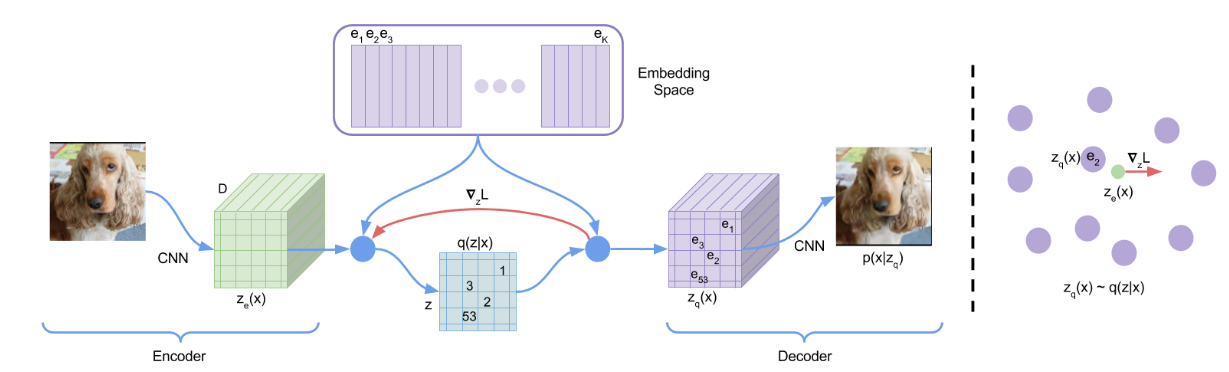
\includegraphics[width=0.9\textwidth]{figures/vq-vae-paper}

sg: stop gradient
\begin{align*}
  L_{VQ-VAE} &= \log p_{\theta}\left(x | Z_q(x)\right) + \Vert Z_e(x) - sg(e_k) \Vert^2_2
               + \underbrace{\Vert sg(Z_e(x)) - e_k \Vert_2^2}_{\text{commitment loss}}\\
\end{align*}

Learning to sample from latent space of VQ-VAE is difficult

\section{Adversarial Learning}
\label{sec:adversarial-learning}

Here, we make a sampler and try to match its output with the given samples. We train a classifier that differentiates the samples from the sampler and the given ones. We try tweaking the sampler until the classifier(all) fails to differentiate. This classifier is called the adversary.

\textbf{Note}: GAN's cannot do posterior inference in their naive form

\vspace{1em}
$\hat{x} = g_{\theta}(z)$ and suppose $p_{\theta}(\hat{x})$ is the distribution of $\hat{x}$ \\
\textbf{Objective}: Make $p_{\theta}(\hat{x})$ close to $p_x$

\ctikzfig{adv_learning_1}

\begin{framed}
  \textbf{Issues with KL}
  \begin{align*}
    \theta_{ML}^{*} &= \arg\min_{\theta} D_{KL}\left( P_X \Vert P_{\theta}  \right) \\
    D_{KL}\left( P_X \Vert P_{\theta} \right) &= \int_X P_X(x) \log \frac{P_X(x)}{P_{\theta}(x)} dx
  \end{align*}

  \begin{minipage}{0.5\textwidth}
    \begin{framed}
      \centering
      Suppose $\tilde{x} \in X$, such that \\
      $P_X(\tilde{x}) \gg P_{\theta}(\tilde{x})$ \\
      This situation is called \\ \textbf{mode dropping / mode collapse} \\
      KL $\uparrow$ (desirable) \\
      KL prevents this by definition
    \end{framed}
  \end{minipage}
  \begin{minipage}{0.5\textwidth}
    \begin{framed}
      \centering
      Suppose $\tilde{x} \in X$, such that \\
      $P_X(\tilde{x}) \ll P_{\theta}(\tilde{x})$ \\
      This situation is called \\ \textbf{garbage/noise generation} \\
      KL $\downarrow$ (not desirable) \\
      KL doesn't prevent this
    \end{framed}
  \end{minipage}
\end{framed}

\subsection{f-divergence Measures}
\label{sec:f-diverg-meas}

Given two distributions $\mathbb{P}$ and $\mathbb{Q}$, with respective absolute continuous density functions $p$ and $q$, defined on the domain $\mathcal{X}$, f-divergence between $\mathbb{P}$ and $\mathbb{Q}$ are defined as 

\begin{align*}
  D_f \left[ \mathbb{P} \Vert \mathbb{Q} \right] = \int_{\mathcal{X}} q(x) f\left( \frac{p(x)}{q(x)} \right)dx
\end{align*}

Where, $f: \mathbb{R}^+ \rightarrow \mathbb{R}$ (generator function) is a convex, lower-semi continuous and $f(1) = 0$

\paragraph{Examples of f-divergences:}
\begin{enumerate}[i)]
\item $f(t) = t \log t$, $t \in \mathbb{R}^+$, $D_f \equiv D_{KL}$
\item $f(t) = - \log t$, $D_f \equiv $ reverse KL
  
\item $f(t) = -(t + 1) \log \frac{(1 + t)}{2} + t \log t$, Jensen-Shanon Divergence
\end{enumerate}

\subsection{Variational f-divergence minimization}
\label{sec:vari-f-diverg}

\textbf{Fenchel conjugate}: Every convex function $f$ has a conjugate $f^{*}$ defined as

\begin{minipage}{0.7\textwidth}
  \begin{align*}
    f^{*}(t) &\triangleq \sup_{u\, \in\, \text{domain}_f} \left\{ ut - f(u) \right\}
  \end{align*}
  Here, $ut - f(u)$ is the lower bound of the function at $t$.
  If the function is convex and the supremum is achievable,
  it becomes the tangent at that point.
\end{minipage}
\begin{minipage}{0.3\textwidth}
  \ctikzfig{fenchel_conjugate_1}
\end{minipage}

\vspace{1em}
\textbf{21st September 2023}

In generative models, we only have access to samples from $P_x$ and $P_{\theta}$ and not
even to the actual $P_{\theta}$. From this we need to estimate $D_f(P_x \Vert P_{\theta})$. That's why we need to get the final term in terms of expectations which can be computed using Monte-Carlo estimates.

\textbf{Note:}
\begin{itemize}
  \item \( f^{*}(t) \text{ is the dual of } f(t)\quad \text{[convex]} \)
  \item \( f^{**} = f \)
\end{itemize}

\begin{align*}
  D_f(p \Vert q) &= \int_{\mathcal{X}} q(x) f \left( \frac{p(x)}{q(x)} \right)dx,
                   \quad\text{let, }u = \frac{p(x)}{q(x)} \\
                 &= \int_{\mathcal{X}} q(x) \sup_{t\, \in\, \text{domain}_{f^{*}}}
                   \underbrace{\left\{ t \frac{p(x)}{q(x)} - f^{*}(t) \right\}}_{O(x, t) \leq O(x, t^{*})}dx \\
  \implies D_f(p \Vert q) &= \sup_{T(x)\, \in\, \mathcal{T}} \underbrace{\int_{\mathcal{X}} q(x)
                            \left\{ T(x) \frac{p(x)}{q(x)} - f^{*}(T(x)) \right\}}_{I_1}
\end{align*}
Here,  $T: \,\mathcal{X} \rightarrow \mathbb{R}(\text{domain } f^{*})$ \\
$T \in \mathcal{T}: $ set of all functions from $ \mathcal{X} \rightarrow \mathbb{R}$,
it is also the set of functions containing the solutions for optimization problem. \\

The $T^{*}$ which would maximize $I_1$, will be the one that \\
is $T^{*}(x) = t^{*}(x)$ for all $x$, where $t^{*}(x) = \sup_tO(x, t)$.

\vspace{1em}
For any $T \in \mathcal{T} \not = T^{*}(x)$,
\begin{align*}
  \sup_{T(x)\, \in\, \mathcal{T}} I_1 &\leq D_f(p \Vert q) \\
  \therefore D_f(p \Vert q) &\geq \sup_{T\, \in\, \mathcal{T}} I_1 \\
  \implies D_f(p \Vert q) &\geq \sup_{T(x)\, \in\, \mathcal{T}} \int_{\mathcal{X}} p(x)T(x)dx
                            - \int_{\mathcal{X}} q(x) f^{*}(T(x))dx \\
  &\geq \sup_{T(x)\, \in\, \mathcal{T}} \left[ \E_P T(x) - \E_Q f^{*}(T(x)) \right]
\end{align*}

\begin{framed}
  Suppose, \\
  $\mathcal{D} = \left\{ x_1, x_2, ..., x_n \right\} \sim \text{i.i.d.} P_x$ \\
  $\mathcal{\hat{D}} = \left\{ \hat{x}_1, \hat{x}_2, ..., \hat{x}_n \right\} \sim \text{i.i.d.} P_{\theta}$

  \vspace{1em}
  \textbf{Objective}: $\min_{\theta} D_f(P_x \Vert P_{\theta})$ equivalently, optimize the lower bound on $D_f$.
  \begin{align*}
    \text{i.e., }\min_{\theta} D_f(P_x \Vert P_{\theta}) = \min_{\theta} \sup_T I_1 = \inf_{\theta} \sup_{\mathcal{T}} I_1 \rightarrow \text{ saddle point problem}
  \end{align*}
\end{framed}

\textbf{Question:} At what $T$ the lowerbound is tight?
\begin{align*}
  I_1 &= \int_{\mathcal{X}} p(x) T(x) dx - \int_{\mathcal{X}} q(x) f^{*}(T(x))dx \\
  &= \int_{\mathcal{X}} \underbrace{\left[ p(x)T(x) - q(x)f^{*}(T(x)) \right] dx}_{L(x, T(x))}
\end{align*}

\begin{align*}
  &\frac{\nabla L}{\nabla T(x)} = 0 \\
  \implies &p(x) - q(x) (f^{*})'(T(x)) = 0 \\
  \implies &(f*)'(T(x)) = \frac{p(x)}{q(x)} \\
  \implies &f' \circ (f')^{*} (T(x)) = f' \left( \frac{p(x)}{q(x)} \right) \\
  \implies &T_{\text{opt}}(x) = f' \left( \frac{p(x)}{q(x)} \right)
\end{align*}

\subsection{Training/Building a sampler via VDM(variational density minimization)}
Given $\mathcal{D} = \left\{ x_1, x_2, ..., x_n \right\} \sim $ i.i.d. $P_x, x \in \mathbb{R}^d$ \\
Consider $Z \sim \mathcal{N}(0, I)$ and a function $g_{\theta}(z), z \rightarrow \mathbb{R}^d$ (neural network).

\begin{figure}[h]
  \centering
  \ctikzfig{gan1}
  \captionof{figure}{Generator and Discriminator NN}
\end{figure}

Parameterize $T(x)$ with another function $V_w: X \rightarrow \text{domain }f^{*}$ (neural network)

\begin{align*}
  \min_{\theta}\max_w \left[ \E_{P_x} T(x) - \E_{P_{\theta}} f^{*}(T(x)) \right] \\
  = \sum_{x_i \in P_x} T(x_i) - \sum_{\hat{x} \in P_{\theta}} f^{*}(T(\hat{x}))
\end{align*}

\vspace{1em}
\textbf{26th September 2023}

\begin{align*}
  D_f(P \Vert Q) &= \int_x q(x) f \left( \frac{P}{Q} \right) dx \\
                   f &: \mathbb{R}^+ \rightarrow \mathbb{R}
\end{align*}

Two neural networks:
\begin{itemize}
\item Parameterize $T_w$ : usual function approximator
\item Parameterize $Q_{\theta}$ : sampling from $Q_{\theta}$
\end{itemize}

\begin{minipage}{0.70\textwidth}
  \begin{align*}
    dim(z) &\ll dim(\hat{x}) \\
    dim(\hat{x}) &= dim(x)
  \end{align*}
\end{minipage}
\begin{minipage}{0.30\textwidth}
		\centering
		\ctikzfig{generator_vdm}
		\captionof{figure}{Generator NN}
      \label{fig:generator_nn}
\end{minipage}

\begin{align*}
  L(\theta, w) &= \E_{x \sim P_x}(T_w(x)) - \E_{\hat{x} \sim Q_{\theta}} \left[ f^{*} (T(\hat{x})) \right]
\end{align*}
Adversarial network

Suppose an $f$-function is chosen,
$T_w(x)$ has to respect the domain constraint

\begin{align*}
  T_w(x) = g_f(V_w(x));\quad &V_w(x) : x \rightarrow \mathbb{R}
  &g_f: \mathbb{R} \rightarrow dom\,f^{*}
\end{align*}




\clearpage

\section{Other Discussions}
\label{sec:other-disc}

\begin{itemize}
\item Probabilistic graphical models (PGM)
\item Manifold hypothesis
  \begin{itemize}
  \item defomorphism example: 2 sets that can be connected by a bijective function
  \item Manifold: $M \subset \mathbb{R}^d$ (ambient space)
  \item Manifold: subset has defomorphism to euclidean subspace
  \item hypothesis: the data lies on a very low dimensional manifold
  \item a subspace is a subset of a manifold (eg: a circle is a manifold but not a subspace)
  \end{itemize}
\item Typewriter monkey problem
\item Ambient space
\item Affine radom variable: scaled and shifted form of a random variable
\item Any random variable can be reparameterized using Gumbel softmax
\item Dirac delta
\item elliptical k-means algorithm
\item Box-Muller method
\end{itemize}

\clearpage
\section{Homework}
\label{sec:homework}

\textbf{10th August 2023}
\begin{enumerate}
\item Define KL divergence between a pair of distribution functions and establish an equivalence between this function and the function described in class.
\item Create a case where KL divergence is valid for distribution functions but not for density functions.
\item Show that KL divergence is not a metric (doesn't hold the triangle equality).
\item Show that KL divergence is always non-negative.
\item Show that KL divergence is zero if and only if when the densities match.
\item Show that KL divergence is not symmetric ($\mathcal{D}_{KL}(P_x || P_{\theta}) \not = \mathcal{D}_{KL}(P_{\theta} || P_x)$).
\item Show that $f(x)$ will not have the same density function as $x$. Find it.
\item Prove LOTUS (Law of the unconscious statistician).
\item Get an ML estimate for the parameter of exponential distribution.
\end{enumerate}

\textbf{17th August 2023}
\begin{enumerate}
\item Show that the ML estimate is unbiased and see whether it is consistent.
\item Formally write the definition of universal density approximation. Why is GMM an example of it?
\end{enumerate}

\textbf{22nd August 2023}
\begin{enumerate}
\item Compute the EM algorithm for GMM and find the closed form parameters.
\item Prove that K-means algorithm is EM. Assume covariances of component gaussions to be diagonal (i.e., $\Sigma = \sigma I$). Show that the reassignment and distance calculation in K-means is same as expectation and maximization in EM algorithm.
\end{enumerate}

\textbf{24th August 2023}
\begin{enumerate}
\item Take a uniform random variable and find the deterministic transformation of it that converts it into a normal random variable. \\($U[0, 1] \rightarrow \mathcal{N}[\mu, \sigma]$)
\end{enumerate}

\textbf{29th August 2023}
\begin{enumerate}
\item Show that gradient is a linear operator.
\item Prove that \( \E_{P_{\psi}(v)} f_{\psi}(v) = \E_{P_{\epsilon}}\left[ f_{\psi}\left( g_{\psi}(\epsilon) \right) \right] \).
\item Show that the distribution of the distribution function of any random variable is uniform between 0 and 1.
\end{enumerate}

\textbf{31st August 2023}
\begin{enumerate}
\item Find the deterministic form of $D_{Kl}\left[ \mathcal{N}(z, \mu_x, \Sigma_x) \Vert \mathcal{N}(z, 0, I) \right]$.
\end{enumerate}

\textbf{5th September 2023}
\begin{enumerate}
\item Show that $D_{KL}\left[ Q_{\phi}(z|x) \Vert P_{\theta}(z|x) \right] = \log P_{\theta}(x) - F_{\theta}(Q_{\phi})$.
\end{enumerate}

\textbf{12th September 2023}
\begin{enumerate}
\item Show that $D_{KL}\left[ q_{\phi}(z|x) \Vert p(z) \right] = \log K$.
\end{enumerate}

\textbf{14th September 2023}
\begin{enumerate}
\item Show that in the case of reverse KL divergence, over-estimation is prevented but under-estimation is not prevented.
\item Show that the $D_f [\mathbb{P} \Vert \mathbb{Q}] = 0$ iff $\mathbb{P} = \mathbb{Q}$.
\item Define f-divergence using the distribution functions and show the equivalence of the distribution is equivalent to the one with density functions if the density functions exist.
\item Argue why $f$ has to be lower-semi continuous and construct a counter example where $f$ is not lower-semi continuous which leads to a undesirable result.
\item Show that $f^{**} = f$.
\end{enumerate}

\textbf{21st September 2023}
\begin{enumerate}
\item Construct 2 examples for \textbf{Euler-Lagrangian} equations.
\item Show that $(f^{*})' = (f')^{*}$.
\end{enumerate}

\textbf{26th September 2023}
\begin{enumerate}
\item Show that $L(\theta, w) = \E_{x \sim P_x} \log D_w(x) + \E_{x \sim Q_{\theta}} \log (1 - D_w(x))$,
  given that \\
  $D_w(x) = \frac{1}{1 + e^{-v_w(x)}} = sigmoid(-v_w(x))$, \\$f^{*}(t) = - \log (1 - e^t)$
  and \\
  $g_f(v) = - \log (1 + e^{-v})$.
\end{enumerate}

\section{TODO}
\label{sec:todo}

\begin{itemize}
\item Read the paper ``ELBO surgery''
\end{itemize}
\end{document}
%%% Local Variables:
%%% mode: latex
%%% TeX-master: t
%%% End:
